% This LaTeX was auto-generated from MATLAB code.
% To make changes, update the MATLAB code and export to LaTeX again.

\documentclass{article}

\usepackage[utf8]{inputenc}
\usepackage[T1]{fontenc}
\usepackage{lmodern}
\usepackage{graphicx}
\usepackage{color}
\usepackage{hyperref}
\usepackage{amsmath}
\usepackage{amsfonts}
\usepackage{epstopdf}
\usepackage[table]{xcolor}
\usepackage{matlab}

\sloppy
\epstopdfsetup{outdir=./}
\graphicspath{ {./training_data_images/} }

\matlabhastoc

\begin{document}

\label{T_5D5AB6FD}
\matlabtitle{Training data }

\matlabtableofcontents{Table of Contents}
\begin{par}
\begin{flushleft}
More on \href{https://github.com/slevin48/gta}{https://github.com/slevin48/gta} 
\end{flushleft}
\end{par}


\label{H_6193C936}
\matlabheading{Data access}

\label{H_73D1E60D}
\matlabheadingtwo{Get images}

\begin{matlabcode}
training_dataset = "2021-03-06-1";
training_data_0 = imread("D:\devel\AI-workflow\samples2\"+training_dataset+"\img_0.png");
imshow(training_data_0)
\end{matlabcode}
\begin{center}
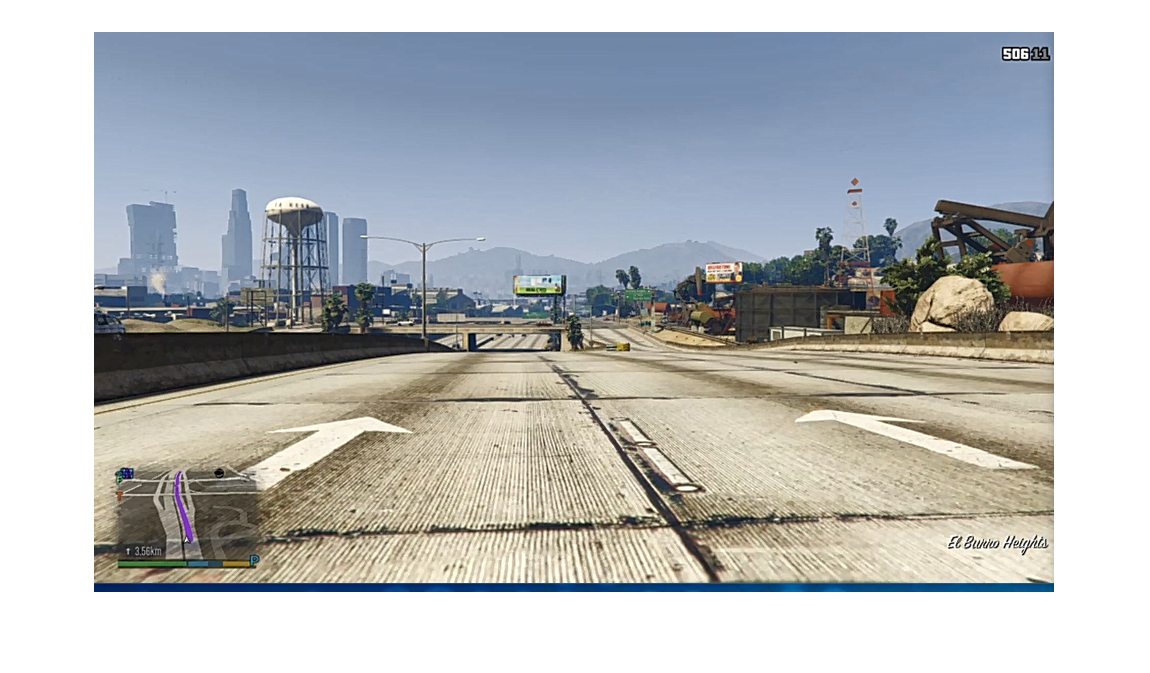
\includegraphics[width=\maxwidth{92.32313095835424em}]{figure_0.png}
\end{center}


\begin{matlabcode}
length(ls("D:\devel\AI-workflow\samples2\"+training_dataset))
\end{matlabcode}
\begin{matlaboutput}
ans = 352
\end{matlaboutput}


\begin{matlabcode}
i = 1;
training_img = imread("D:\devel\AI-workflow\samples2\"+training_dataset+"\img_"+string(i)+".png");
imshow(training_img)
\end{matlabcode}
\begin{center}
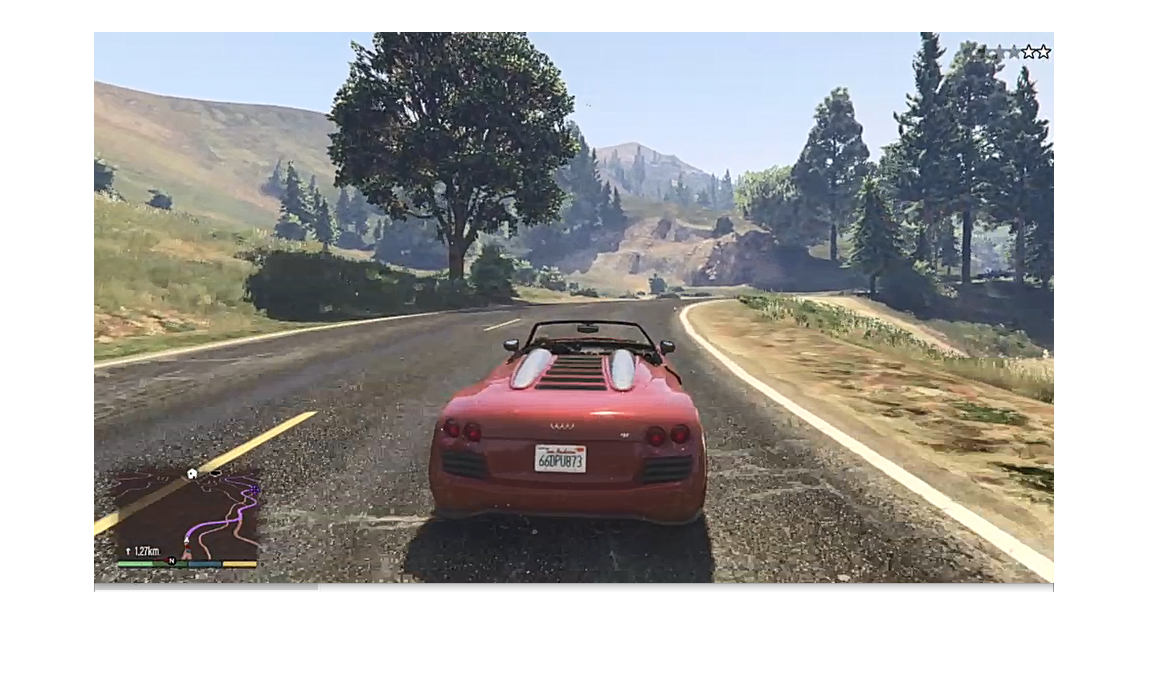
\includegraphics[width=\maxwidth{92.32313095835424em}]{figure_1.png}
\end{center}


\label{H_6D71882E}
\matlabheadingtwo{Get controller data}

\begin{matlabcode}
data = readtable("D:\devel\AI-workflow\samples2\"+training_dataset+"\data.csv");
data = renamevars(data,["Var1","Var2","Var3","Var4","Var5","Var6"],["img", "x", "y", "r", "l", "b"]);
data
\end{matlabcode}
\begin{matlabtableoutput}
{
\begin{tabular} {|c|c|c|c|c|c|c|}\hline
\mlcell{ } & \mlcell{img} & \mlcell{x} & \mlcell{y} & \mlcell{r} & \mlcell{l} & \mlcell{b} \\ \hline
\mlcell{1} & \mlcell{'samples/2021-03-06-1/img\_0.png'} & \mlcell{-0.0157} & \mlcell{-0.0079} & \mlcell{0} & \mlcell{0} & \mlcell{0} \\ \hline
\mlcell{2} & \mlcell{'samples/2021-03-06-1/img\_1.png'} & \mlcell{-0.0157} & \mlcell{-0.0157} & \mlcell{0} & \mlcell{0} & \mlcell{0} \\ \hline
\mlcell{3} & \mlcell{'samples/2021-03-06-1/img\_2.png'} & \mlcell{-0.0157} & \mlcell{-0.0079} & \mlcell{0} & \mlcell{0} & \mlcell{0} \\ \hline
\mlcell{4} & \mlcell{'samples/2021-03-06-1/img\_3.png'} & \mlcell{-0.0157} & \mlcell{-0.0079} & \mlcell{0} & \mlcell{0} & \mlcell{0} \\ \hline
\mlcell{5} & \mlcell{'samples/2021-03-06-1/img\_4.png'} & \mlcell{-0.0236} & \mlcell{-0.0079} & \mlcell{0} & \mlcell{0} & \mlcell{0} \\ \hline
\mlcell{6} & \mlcell{'samples/2021-03-06-1/img\_5.png'} & \mlcell{-0.0157} & \mlcell{-0.0079} & \mlcell{0} & \mlcell{0} & \mlcell{0} \\ \hline
\mlcell{7} & \mlcell{'samples/2021-03-06-1/img\_6.png'} & \mlcell{-0.0157} & \mlcell{-0.0079} & \mlcell{0} & \mlcell{0} & \mlcell{0} \\ \hline
\mlcell{8} & \mlcell{'samples/2021-03-06-1/img\_7.png'} & \mlcell{-0.0157} & \mlcell{-0.0079} & \mlcell{0} & \mlcell{0} & \mlcell{0} \\ \hline
\mlcell{9} & \mlcell{'samples/2021-03-06-1/img\_8.png'} & \mlcell{-0.0157} & \mlcell{-0.0157} & \mlcell{0} & \mlcell{0} & \mlcell{0} \\ \hline
\mlcell{10} & \mlcell{'samples/2021-03-06-1/img\_9.png'} & \mlcell{-0.0157} & \mlcell{-0.0079} & \mlcell{0.9961} & \mlcell{0} & \mlcell{0} \\ \hline
\mlcell{11} & \mlcell{'samples/2021-03-06-1/img\_10.png'} & \mlcell{-0.0157} & \mlcell{-0.0157} & \mlcell{0.9961} & \mlcell{0} & \mlcell{0} \\ \hline
\mlcell{12} & \mlcell{'samples/2021-03-06-1/img\_11.png'} & \mlcell{-0.0394} & \mlcell{-0.0079} & \mlcell{0.9961} & \mlcell{0} & \mlcell{0} \\ \hline
\mlcell{13} & \mlcell{'samples/2021-03-06-1/img\_12.png'} & \mlcell{-0.0709} & \mlcell{-0.0157} & \mlcell{0.9961} & \mlcell{0} & \mlcell{0} \\ \hline
\mlcell{14} & \mlcell{'samples/2021-03-06-1/img\_13.png'} & \mlcell{-0.2047} & \mlcell{-0.0157} & \mlcell{0.9961} & \mlcell{0} & \mlcell{0} \\ 
\hline
\end{tabular}
}
\end{matlabtableoutput}


\begin{matlabcode}
plot(data.x)
\end{matlabcode}
\begin{center}
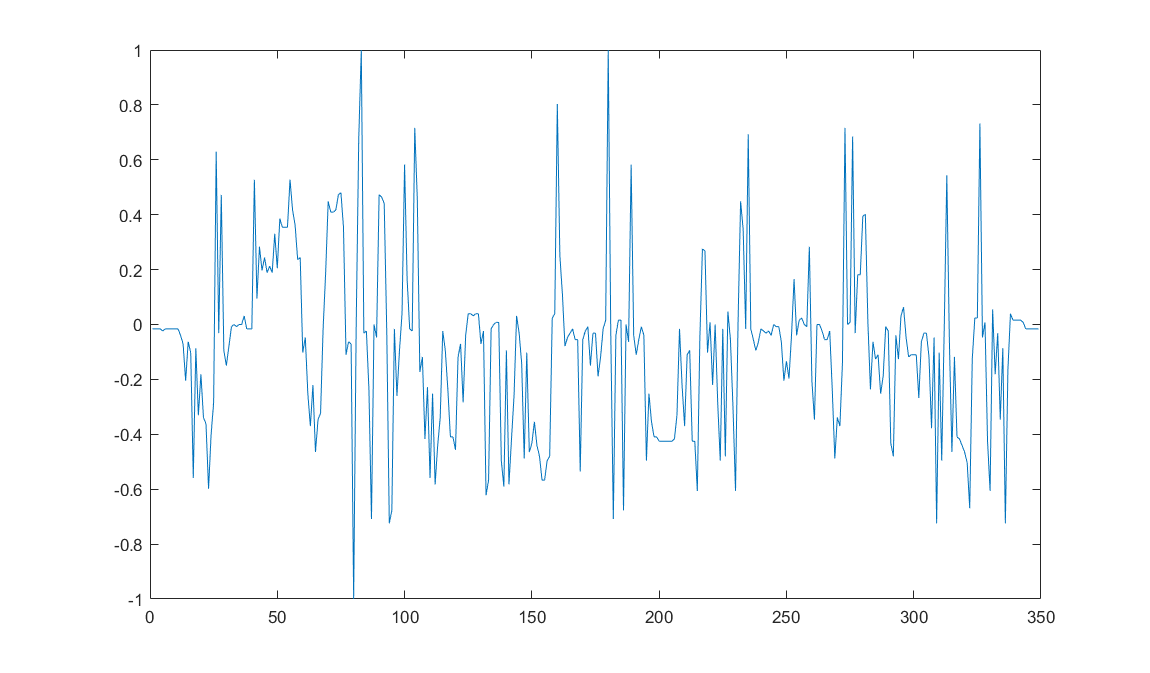
\includegraphics[width=\maxwidth{92.32313095835424em}]{figure_2.png}
\end{center}


\label{H_2996B159}
\matlabheadingtwo{Get data from Numpy directly}

\begin{matlabcode}
pyenv
\end{matlabcode}


\begin{matlabcode}
training_dir = uigetdir
% training_dataset"training_data-2021-02-12-2"
% training_dir = "training_data\"+training_dataset
\end{matlabcode}


\begin{matlabcode}
npfiles = dir(training_dir+"\*.npy")
length(npfiles)
\end{matlabcode}


\begin{matlabcode}
% npdata = py.training_data.load_data(training_dir+"/X.npy")
\end{matlabcode}


\label{H_8263E867}
\matlabheadingtwo{Browse training data with an app}

\begin{par}
\begin{flushleft}
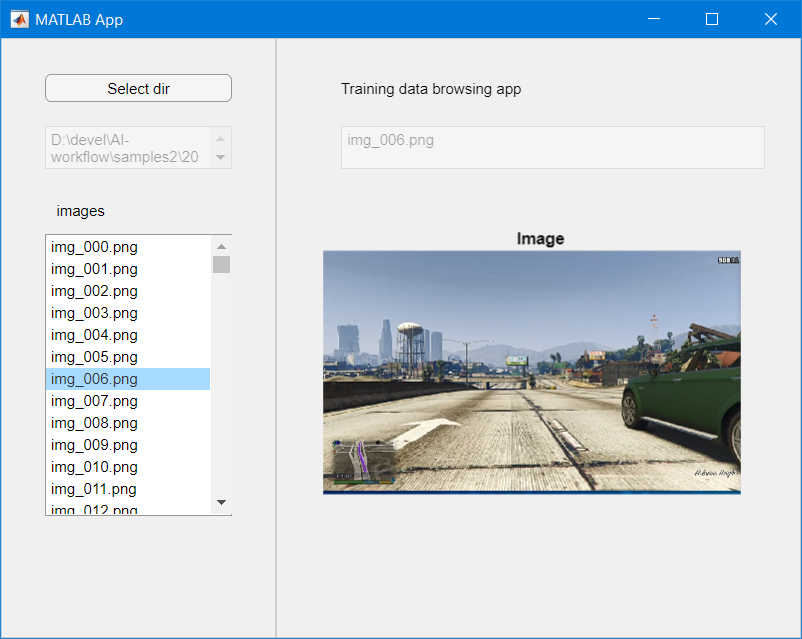
\includegraphics[width=\maxwidth{59.80933266432514em}]{image_0}
\end{flushleft}
\end{par}


\label{H_E93D3605}
\matlabheadingtwo{Specify data}

\begin{matlabcode}
training_dataset = "2021-03-06-1";
dataFolder = "D:\devel\AI-workflow\samples2\"+training_dataset;
% renameImages(dataFolder); % only need to be run once
imds = imageDatastore(dataFolder);
\end{matlabcode}


\label{H_796969A7}
\matlabheading{Modelling}

\label{H_DD03D0CD}
\matlabheadingtwo{Aside : what does a pre-trained ACF detector give us ?}

\begin{matlabcode}
detector = vehicleDetectorACF('full-view'); % use front-rear-view on highway scenario
vp = vision.VideoPlayer ;

reset(imds);
reset(vp)
while hasdata( imds )
    I = read( imds );
    [bboxes,scores] = detect(detector,I);
    if ~isempty( bboxes )
        I = insertObjectAnnotation(I,'rectangle',bboxes,scores);
    end
    step( vp, I )
    drawnow
end 
\end{matlabcode}
\begin{center}
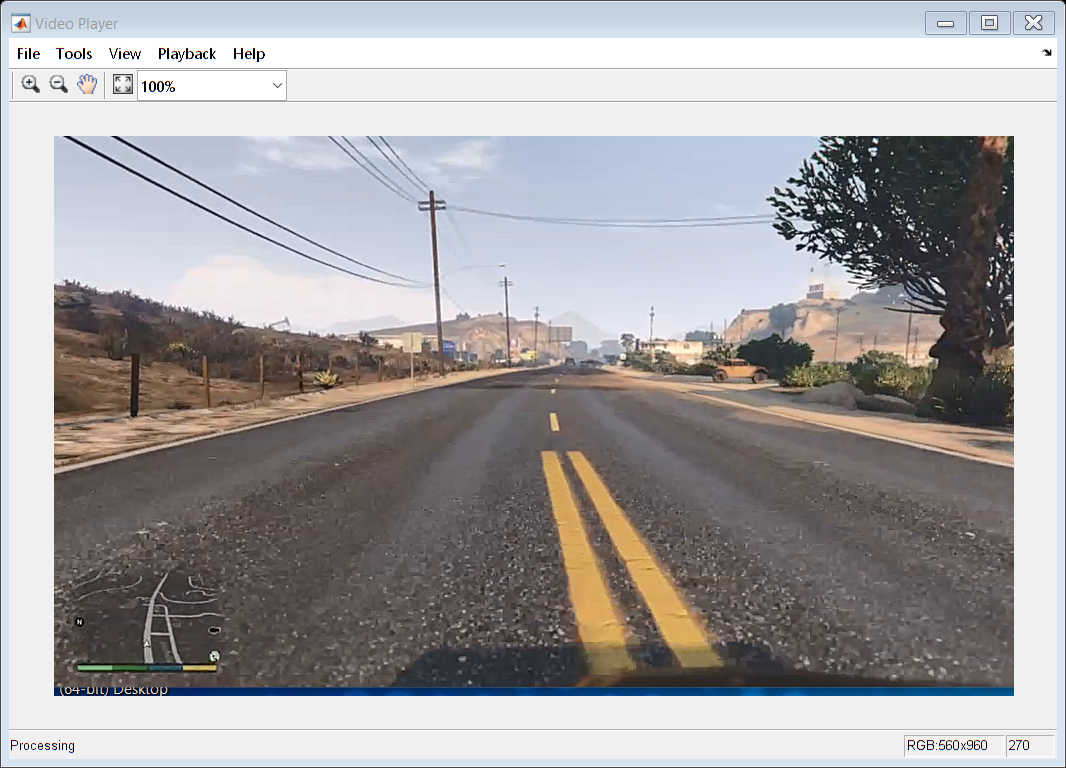
\includegraphics[width=\maxwidth{41.14400401404917em}]{figure_3.png}
\end{center}


\label{H_A0BE5C70}
\matlabheadingtwo{Deep Learning}

\begin{par}
\begin{flushleft}
Read in response data and reformat 
\end{flushleft}
\end{par}

\begin{matlabcode}
training_dataset = "training_data-2021-02-14-1";
sequence = 1;
T = readtable("keyboard/"+training_dataset+"/training_data-"+string(sequence)+".csv");
numPoints = size(T, 1);
right = T.D ;
left = T.Q ;
straight = double(~( logical( right) | logical(left) ));
labels = straight + 2*left + 3*right; 
% onehotencode()
imds.Labels = categorical(labels);
\end{matlabcode}

\begin{par}
\begin{flushleft}
Resize input data to match network architecture
\end{flushleft}
\end{par}

\begin{matlabcode}
outputSize = [270 480];
auimds = augmentedImageDatastore(outputSize, imds);
\end{matlabcode}


\label{H_A1BD8BBE}
\matlabheadingtwo{Use Deep Network Designer to do transfer learning}

\begin{par}
\begin{flushleft}
In this case, using AlexNet for transfer learning does not work as the training is not converging. We need more data, and also to revisit how the problem is formulated. 
\end{flushleft}
\end{par}

\begin{par}
\begin{flushleft}
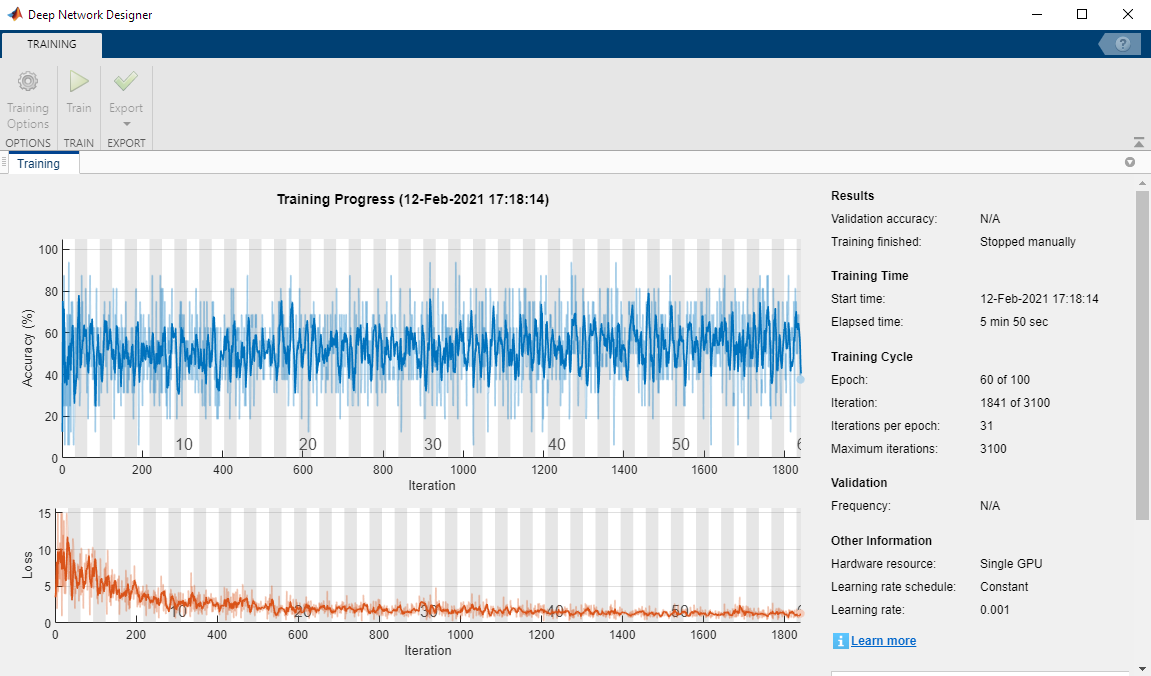
\includegraphics[width=\maxwidth{80.6823883592574em}]{image_1}
\end{flushleft}
\end{par}


\label{H_AAA187D4}
\matlabheadingtwo{Helper function}

\begin{matlabcode}
function renameImages( dataFolder )

D = dir(dataFolder);
nameRoot = "img_";
for i = 4:numel(D) 
%   1 = .    
%   2 = ..
%   3 = data.csv
    if D(i).isdir == 0
        
        I = imread(fullfile(dataFolder, D(i).name));
        [~,filename,ext] = fileparts(D(i).name);
        nameLength = length( filename );
        if nameLength == 7
            continue;
        else
            if nameLength == 5
                imNumber = ["00" + filename(5)] ;
            elseif nameLength == 6
                imNumber = ["0" + filename(5:6)];                
            end
            newFilename = [nameRoot + imNumber + ext];
            imwrite(I, fullfile(dataFolder, newFilename));
            delete(fullfile(dataFolder, D(i).name));
        end
    end
end
end
\end{matlabcode}

\end{document}
